\documentclass[]{article} 
\usepackage{proceed2e}
\usepackage{subfigure}
\usepackage[numbers,sort]{natbib}
\usepackage{amsmath}
\usepackage{amssymb}
\usepackage{graphicx}
\usepackage{ifthen,version}
\newboolean{include-notes}
\usepackage{algorithm}
\usepackage{algpseudocode}
\usepackage[usenames,dvipsnames]{color}
\newcommand{\stnote}[1]{\textcolor{Blue}{\textbf{ST: #1}}}
\newcommand{\jmnote}[1]{\textcolor{Green}{\textbf{JM: #1}}}



\title{Planning with Affordances}

\begin{document}
\author{}
\maketitle

\begin{abstract}
%Current methods for decision-making under uncertainty require
%exhaustive enumeration of all possible states and actions, leading to
%exponential run times caused by 

Planning algorithms for non-deterministic domains are often
intractable in large state and action spaces due to the well-known
``curse of dimensionality.''  Approaches to address this problem by
providing the system with formally encoded knowledge such as
macro-actions and options still fail to prevent the system from
considering many actions which would be obviously irrelevant to a
human solving the same problem.  To address this issue, we introduce a
novel approach which represents knowledge about the domain in terms of
{\em affordances}~\citep{gibson77}.  Our affordance formalism and
associated planning framework allows an agent to efficiently prune its
action space based on domain knowledge.  This pruning significantly
reduces the number of state/action pairs the agent needs to evaluate
in order to act optimally.  We demonstrate our approach in the
Minecraft domain on several planning and building tasks, showing a
significant increase in speed and reduction in state-space exploration
compared to subgoal (partial order) planning.

% options, and macro actions
\end{abstract}

%\stnote{High level things we should add:
%\begin{itemize}
%\item Runtime of the three algorithms in big O notation.
%\item Results with non-deterministic T.
%\end{itemize}
%}

\section{INTRODUCTION}

As robots move out of the lab and into the real world, planning
algorithms need to scale to domains of increased noise, size, and
complexity.  A classic formalization of this problem is a stochastic
sequential decision making problem in which the agent must find a
policy (a mapping from states to actions) for some subset of the state
space that enables the agent to achieve a goal from some initial
state, while minimizing any costs along the way.
%A classic formalization of this issue is the
%sequential decision making problem, where 
Increases in planning problem size
and complexity directly correspond to an explosion in the state-action
space. Current approaches to solving sequential decision making
problems cannot tackle these problems as the state-action space
becomes too large~\citep{grounds05}.

To address this state-space explosion, prior work has explored adding
knowledge to the planner to enable it to solve problems in these
massive domains. However prior approaches such as options and
macro-actions work by providing additional high-level actions to the
agent, which {\em increases} the size of the state/action space (while
also allowing the agent to search more deeply within the space).  The
resulting augmented space is even larger, which can have the
paradoxical effect of increasing the search time for a good policy.

\begin{figure}
\centering
%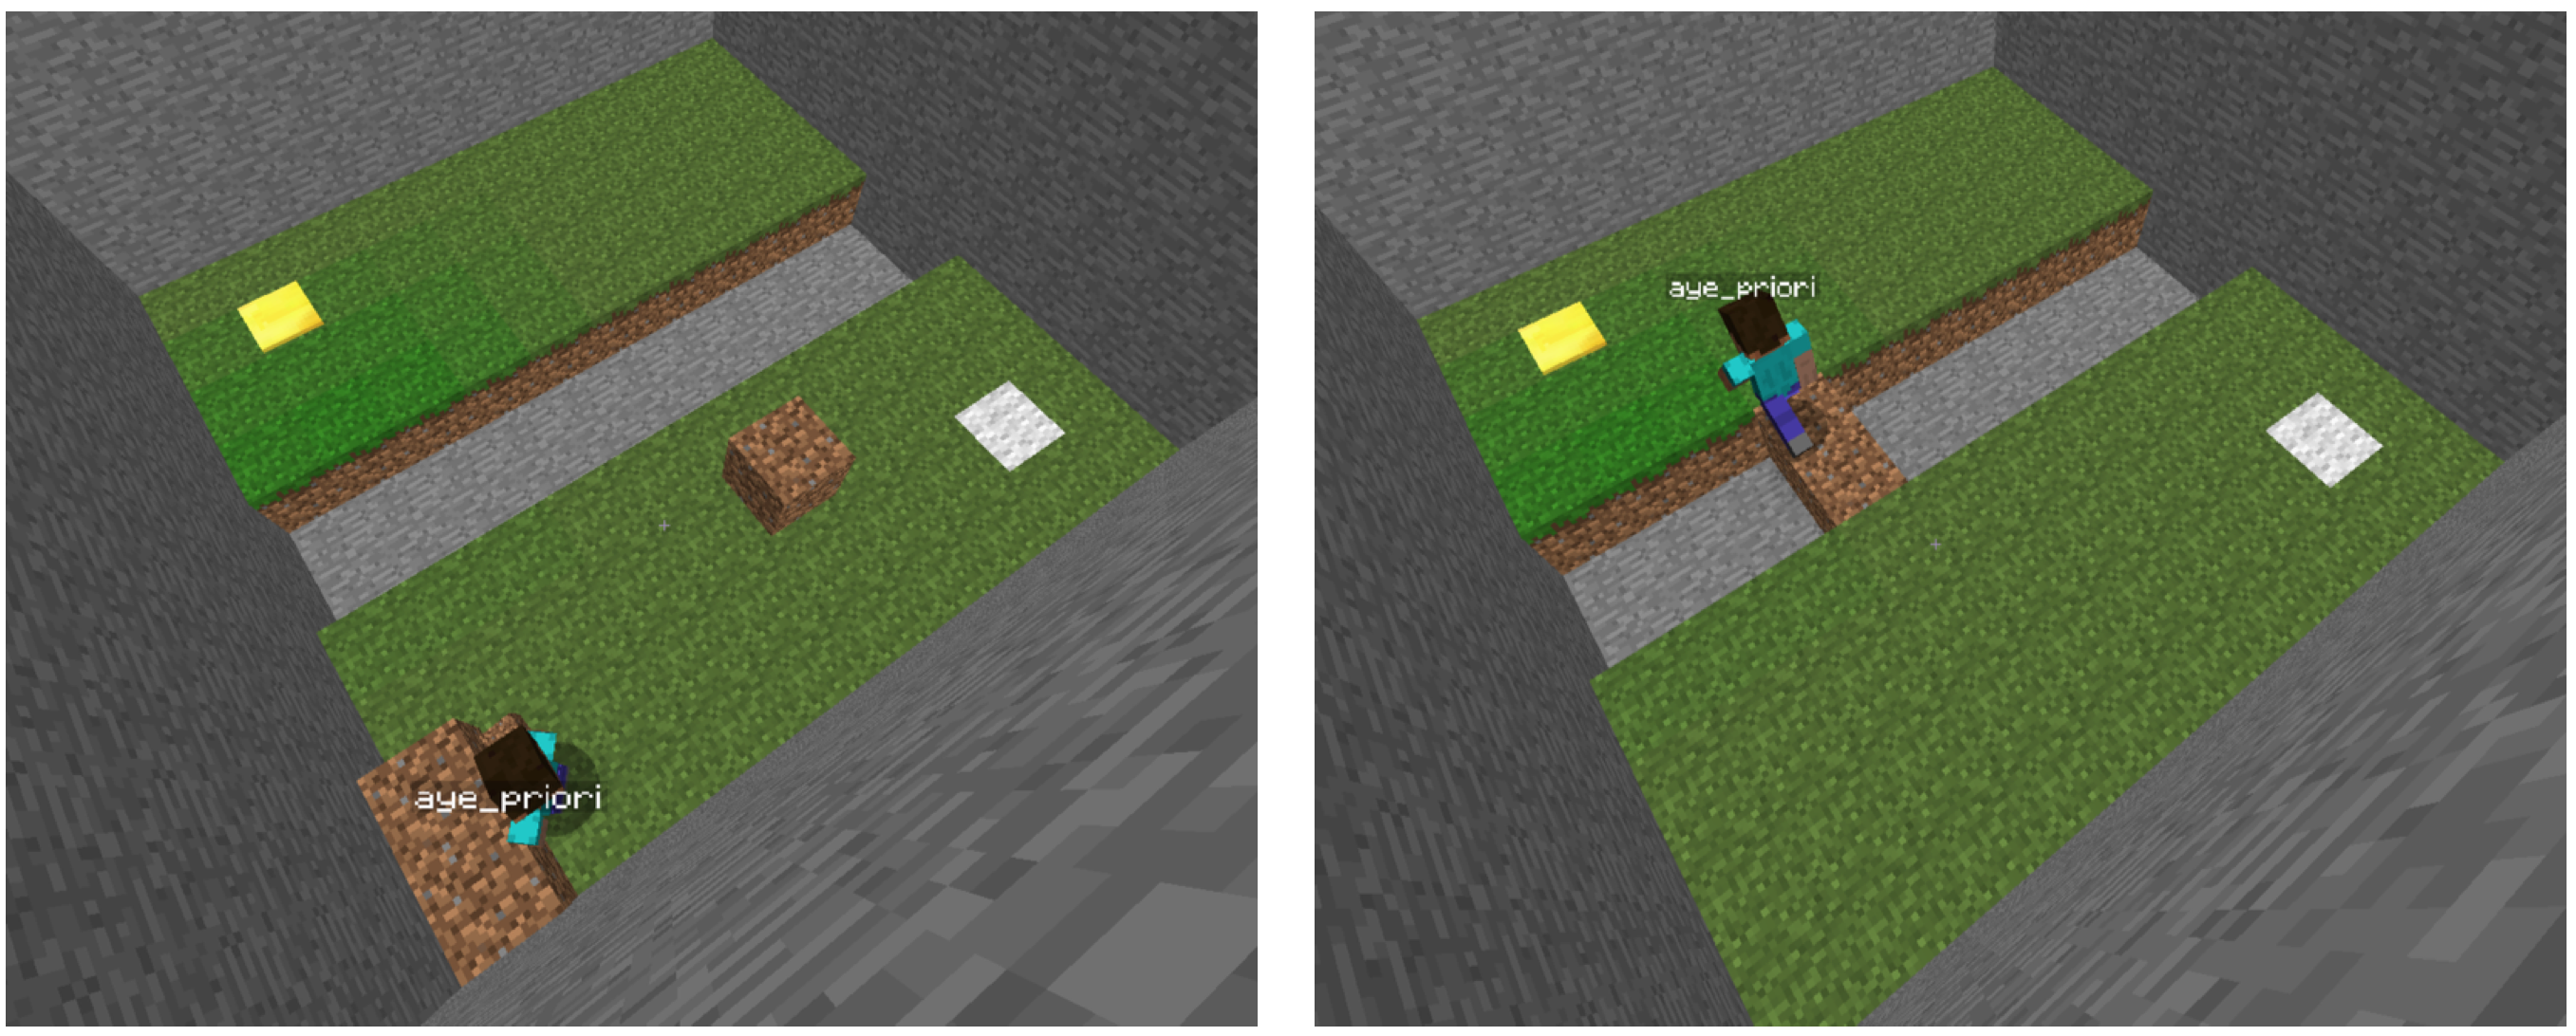
\includegraphics[scale=0.18]{figures/bridgeworld_vi_vs_aff.png}
\subfigure[Planning with VI.]{
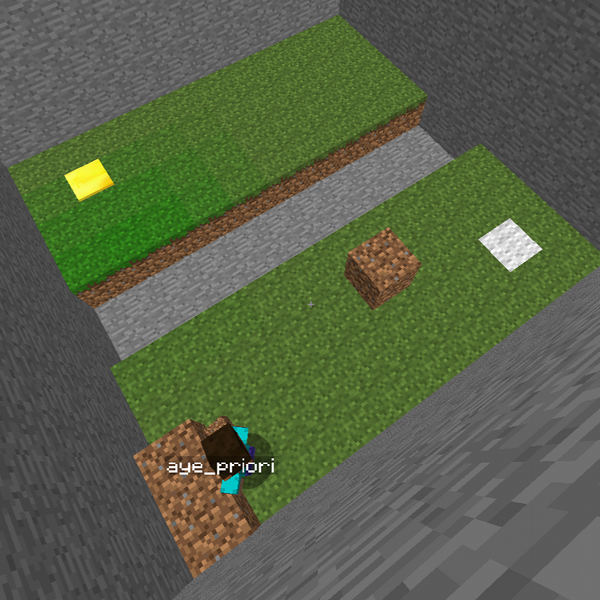
\includegraphics[width=0.5\linewidth]{figures/fig_1_vi_cropped.png}}%
\subfigure[Planning with affordances.]{
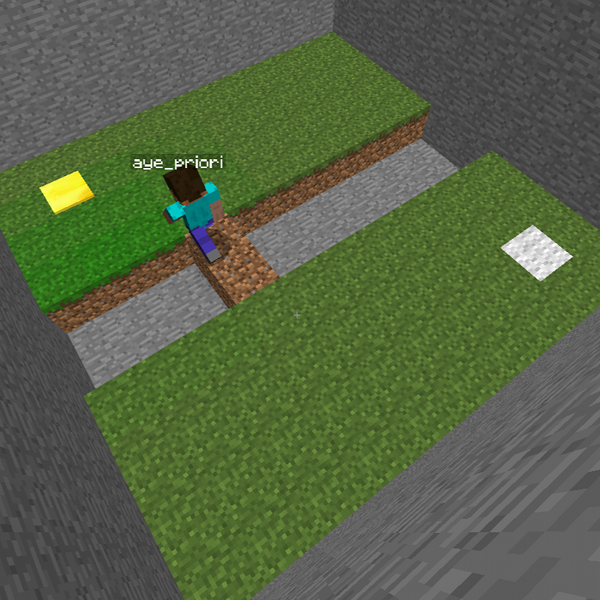
\includegraphics[width=0.5\linewidth]{figures/fig_1_aff_cropped.png}}%
  \caption{Scenes from a Minecraft agent planning using Value
    Iteration (VI) compared to the affordance planner in a bridge
    building task.  VI considers states which would be obviously
    irrelevant to a human solving the same problem, such as stacking
    blocks in the corner.  Our affordance agent, in contrast, focuses
    on placing blocks in the trench, which are much more relevant to
    reaching the goal.\label{fig:minecraft}}
\end{figure}

We propose to address this planning problem by focusing on
problem-specific aspects of the environment which focus the search
toward the most relevant and useful parts of the state-action space.
This approach aims to {\em reduce} the size of the explored state
action space, leading to dramatic speedups in planning.  Our approach
is a formalization of {\em affordances}, introduced by
\citet{gibson77} as ``what [the environment] offers [an] animal, what
      [the environment] provides or furnishes, either for good or
      ill.''  We formalize the notion of an affordance as a piece of
      planning knowledge provided to an agent operating in a Markov
      Decision Process (MDP). We explain how affordances can be
      leveraged by a variety of planning algorithms to prune the
      action set the agent uses dynamically based on the agent's
      current goal.  We call any planning algorithm that uses
      affordances to prune the action set an affordance-aware planning
      algorithm.  A useful property of affordances is that they are
      not specific to a particular reward function or goal, and thus,
      provide the agent with transferable knowledge that is effective
      in a wide variety of problems.

%~\citep{kaelbling99} -- (JM: I don't think you should cite this. This paper involves
%partially observable markov decision processes, which this work does not evaluate.)

%We demonstrate that, like
%an option or macro-action, an affordance provides additional
%information to the agent, enabling more transferable and efficient
%planning.  However, unlike previous approaches, an affordance enables
%more significant speedups by reducing the branching-factor of
%the search space, enabling an agent to focus its search on the most
%relevant part of the problem at hand.  This approach means that a
%single set of affordances provides general domain knowledge, becoming
%relevant just when the agent reasons that it needs to pursue a
%particular goal.  Furthermore, affordances are not specific to a
%particular reward function or goal, and thus, provide the agent with
%transferrable knowledge that is effective in a wide variety of
%problems.


\jmnote{Need to augment this description with the embedded
  stochasticity. If the stochasticity is effectively a probability of
  taking the wrong action/movement, we should relate it the fact that
  in robotics, actuators are noisy and often fail, thereby making the
  domain a bit more analogous to physical robots. We should also
  highlight that this stochasticity can affect the policy by forcing
  the agent to be more cautious in dangerous environments.}  

We use Minecraft as our planning and evaluation domain. Minecraft is a
3-D blocks world game in which the user can place and destroy blocks
of different types.  Minecraft players have constructed complex
worlds, including models of a scientific graphing
calculator~\footnote{https://www.youtube.com/watch?v=wgJfVRhotlQ};
scenes from a Minecraft world appear in Figure~ref{fig:minecraft}.  As a
running example, we will consider the problem of an agent attempting
to cross a trench in a $4 \times 4 \times 2$ Minecraft world shown in
Figure~\ref{fig:bridgeworld}. The floor (at $z = 1)$ \footnote{The
  $z$-axis is the height of the Minecraft world. Similarly, the
  $x$-axis is its width and the $y$-axis is its length.} is composed
of 8 solid blocks, with horizontal empty trenches at $y = 2$ and $y =
3$. The agent is at the starting location $(1, 1, 2)$ and needs to
reach the goal at $(4,4,2)$

To solve the problem, the agent must place a block in the trench to
form a bridge, then cross the bridge to reach the goal.  This task is
challenging for planning algorithms to solve because the reachable
state space in Minecraft is so large. For example, the number of
places an agent can place and destroy blocks alone can result in a
combinatorial explosion of the state space. Specifically, given an
agent capable placing and destroying blocks in a 10x10x2 world, there
are on the order of
\begin{align}
O\left(\sum_{n=1}^{10 \cdot 10 \cdot 2} \binom{10 \cdot 10 \cdot 2}{n}\right)
\label{eq:mc_explode}
\end{align}
states, which is too large for a planning algorithm to explore in a
reasonable time.

%However, when running an uninformed planning
%technique such as value iteration, the agent must enumerate all
%possible states, such as placing a block in the corner and
%subsequently destroying it.  Considering these actions (which are
%obviously irrelevant to a human player) results in a combinatoric
%explosion of the state space (see Equation \ref{eq:mc_explode}).


\section{BACKGROUND}

We define affordances in terms of propositional functions on states.
Our definition builds on the Object-Oriented Markov Decision Process
(OO-MDP)~\citep{diuk08}.  OO-MDPs~\citep{diuk08} are an extension of
the classic Markov Decision Process (MDP).  A classic MDP is a
five-tuple: $\langle \mathcal{S}, \mathcal{A}, \mathcal{T},
\mathcal{R}, \gamma \rangle$, where $\mathcal{S}$ is a state-space;
$\mathcal{A}$ is the agent's set of actions; $\mathcal{T}$ denotes
$\mathcal{T}(s' \mid s,a)$, the transition probability of an agent
applying action $a \in \mathcal{A}$ in state $s \in \mathcal{S}$ and
arriving in $s' \in \mathcal{S}$; $\mathcal{R}(s,a,s')$ denotes the
reward received by the agent for applying action $a$ in state $s$ and
and transitioning to state $s'$; and $\gamma \in [0, 1)$ is a discount
  factor that defines how much the agent prefers immediate rewards
  over distant rewards (the agent more greatly prefers to maximize
  more immediate rewards as $\gamma$ decreases).

\begin{figure}
\centering
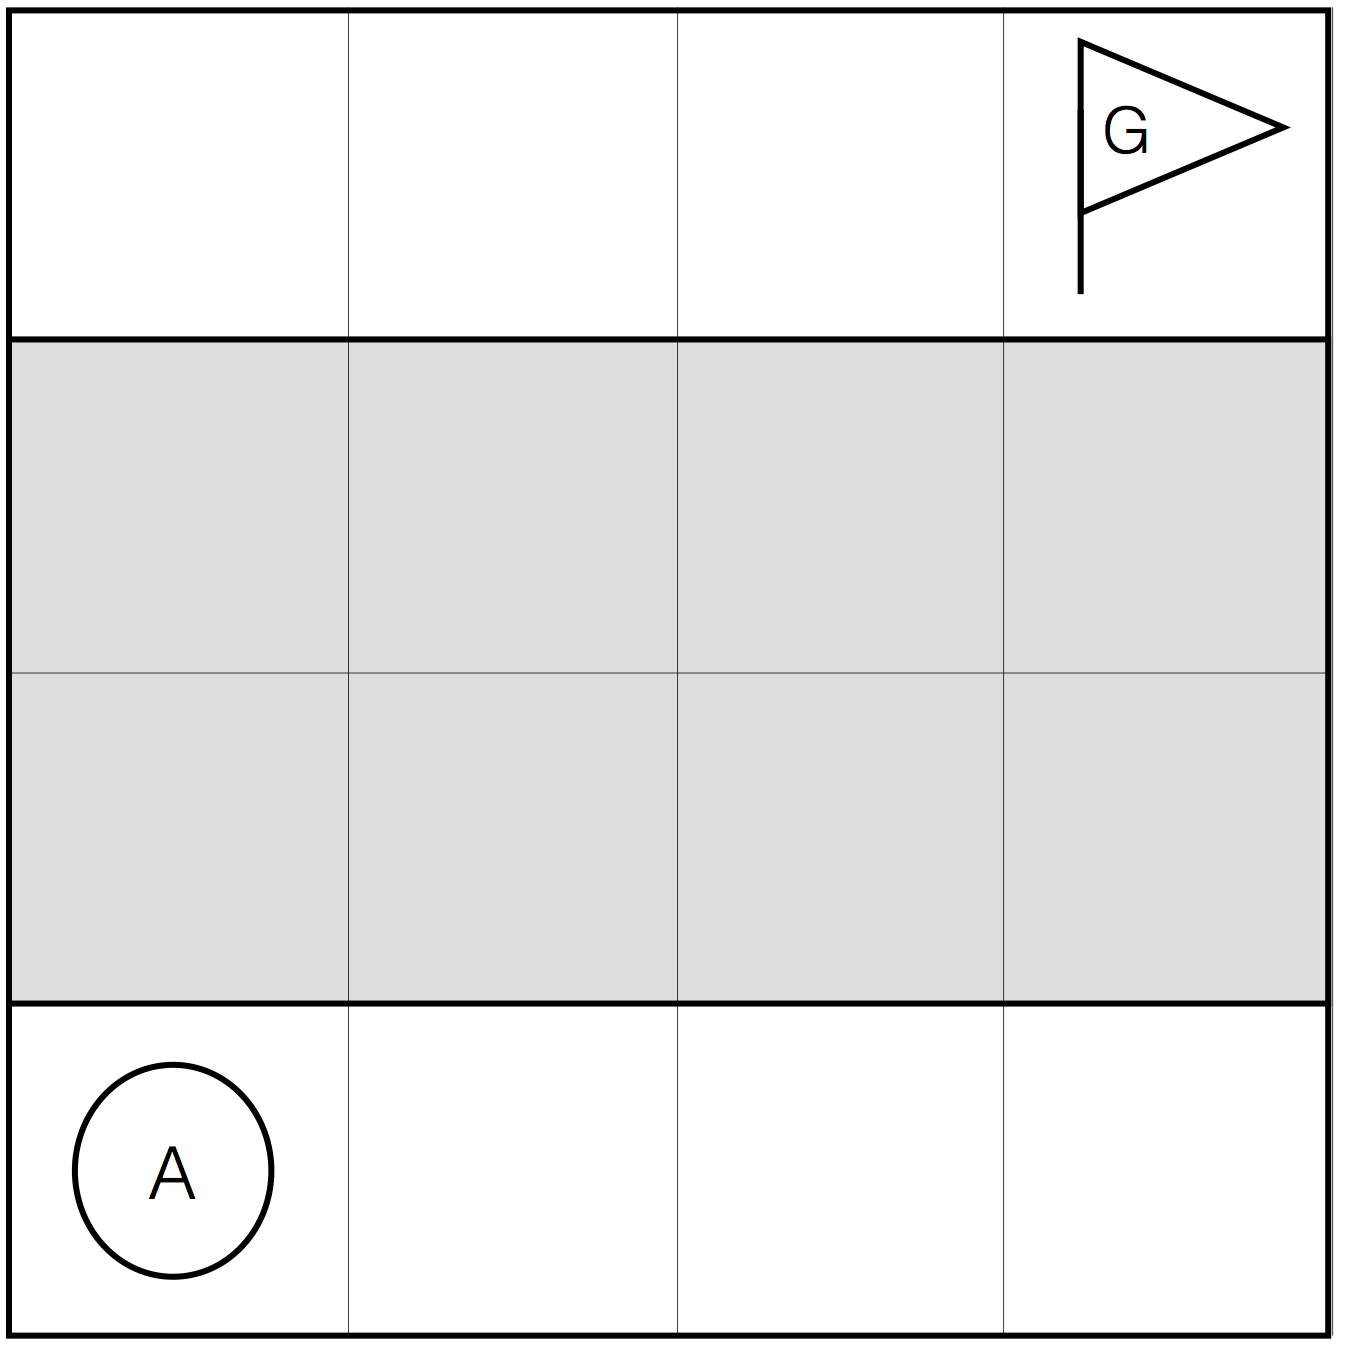
\includegraphics[scale=0.2]{figures/bridgeworld.png}
\caption{In the above Minecraft planning problem \texttt{BRIDGEWORLD},
the agent must place a block in the trench in order to reach the goal 
(the trench is too wide to jump over). \label{fig:bridgeworld}}
\end{figure}


\begin{figure}
\centering
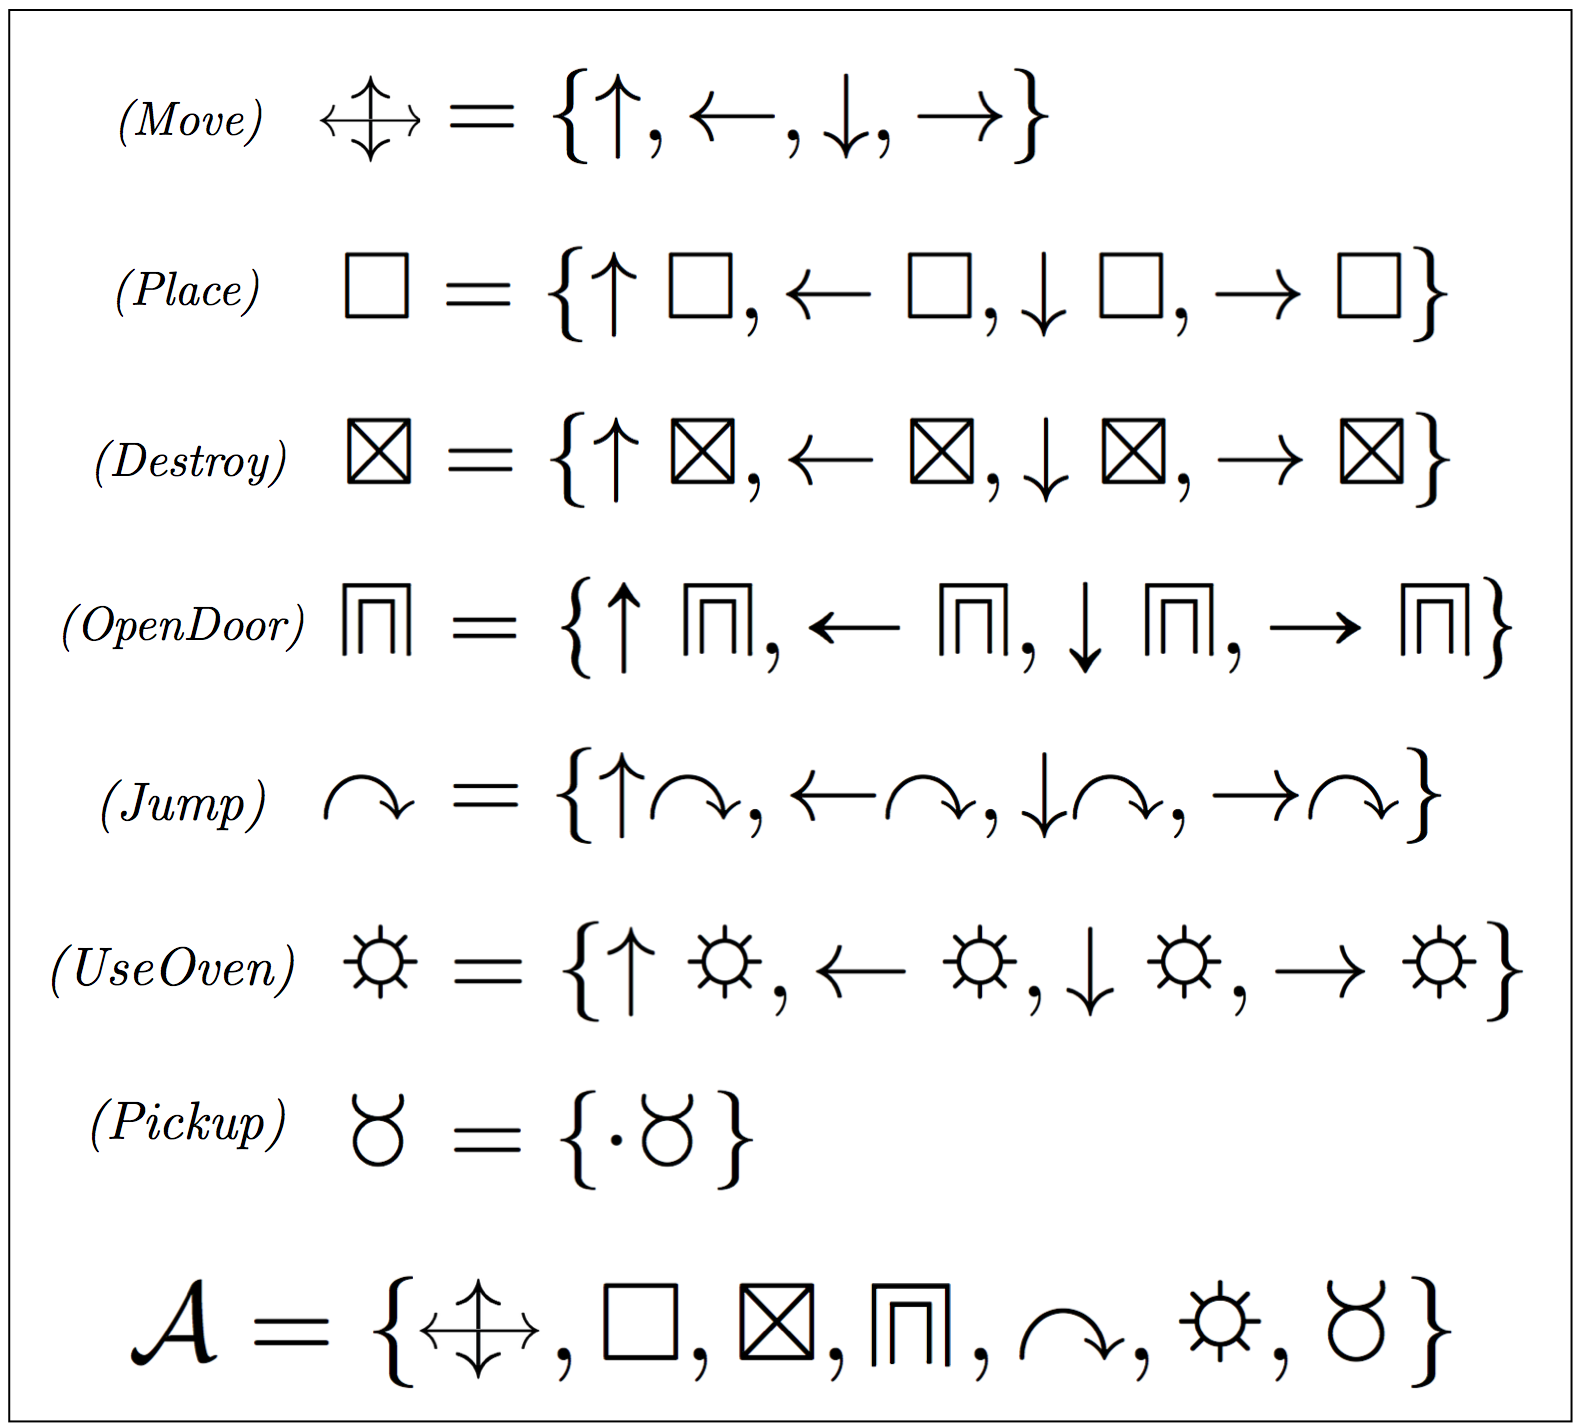
\includegraphics[scale = 0.15]{figures/all_actions.png}
\caption{The set of all actions in the Minecraft domain. \label{fig:all_actions}}
\end{figure}



A classic way to provide a factored representation of an MDP state is to represent
each MDP state as a single feature vector. In contrast, an OO-MDP represents the state space as a collection of objects,
$O = \{o_1, \ldots, o_o \}$.  Each object $o_i$ belongs to a
class $c_j \in  \{c_1, \ldots, c_c\}$. Every class has a set of attributes
$Att(c) = \{c.a_1, \ldots, c.a_a \}$, each of which has a domain $Dom(c.a)$.
Upon instantiation of an object class, its attributes are given a state $o.state$
(an assignment of values to its attributes).  The underlying MDP state is the set
of all the object states: $s \in {\cal S} = \cup_{i = 1}^o \{o_i.state\}$.

There are two advantages to using an object-oriented factored state
representation instead of a single feature vector. First, different
states in the same state space may contain different numbers of
objects of varying classes, which is useful in domains like Minecraft
in which the agent can dynamically add and remove blocks to the
world. Second, MDP states can be defined invariantly to the specific
object references.  For instance, consider a Minecraft world with two
block objects, $b_1$ and $b_2$.  If the agent picked up and swapped
the position of $b_1$ and $b_2$ (and then returned to the agent's
previous position in the world), the MDP state before the swap and
after the swap would be the same, because the MDP state definition is
invariant to which object holds which object state.  Formally, if
there exists a bijection between two sets of objects that maps each
object in one set to an object in the other set with the same object
state, then the two sets of objects define the same MDP state.  This
object reference invariance results in a smaller state space compared
to representations like feature vectors in which changes to value
assignments always result in a different state.

While the OO-MDP state definition is a good fit for the Minecraft
domain, our motivation for using an OO-MDP lies in the ability to
formulate predicates over classes of objects. That is, the OO-MDP
definition also includes a set of predicates ${\cal P}$ that operate
on the state of objects to provide additional high-level information
about the MDP state. For example, in the Minecraft domain, an ${\tt
  on}({\tt BLOCK, BLOCK})$ predicate operates on two objects belonging
to class ${\tt BLOCK}$; ${\tt on}(b_1,b_2)$, would evaluate to true
when the $z$ position value of $b_1$'s state is one unit higher than
the $z$ position value of $b_2$'s, and false otherwise.  \jmnote{This
  should probably be replaced with an example of a predicate that is
  actually used in the Minecraft domain.}  \stnote{I agree -- can we
  use predicates that are relevant to bridgeworld?  Is moveable?  is
  placeable?} In the original OO-MDP work, these predicates were used
to model and learn an MDP's transition dynamics. In the next section,
we use the predicates to define affordances that enable planning
algorithms to prune irrelevant actions.


% As we will
%see in section 3, this helps us form preconditions and goals that
%generalize beyond a particular instance of a state space.

%As with a classical finite MDP, planning with an OO-MDP involves
%running value iteration to determine a policy.  Reward propagation in
%value iteration occurs as in a Bellman update:
%\begin{align}
%U_{i+1}(s) \leftarrow \mathcal{R}(s) + \gamma \max_{a \in \mathcal{A}(s)} \sum_{s'} \text{Pr}(s' \mid s, a)U_i(s')
%\end{align}
%Where $U_i(s)$ is the {\it utility} of state $s$ at iteration $i$, 
%representing the expected reward of being in that state. See Algorithm \ref{alg:vi} for the full pseudocode of the algorithm ~\citep{russellnorvigAI}.%

%% VI pseudocode from Norvig/Russell
%\begin{algorithm}
%  \caption{Value-Iteration($\mathcal{A}$, $\mathcal{R}$, $\mathcal{S}$, $\epsilon$, $\gamma$) \\ {\it Complexity:} $\mathcal{O}(|\mathcal{A}|\cdot |\mathcal{S}|^2)$}
%  \begin{algorithmic}[1]
%    \While {$\delta < \epsilon \frac{(1-\gamma)}{\gamma}$}
%    \State $U \gets U';\delta \gets 0$
%    \For {each state $s \in \mathcal{S}$}
%    \State $U'[s] \leftarrow \mathcal{R}(s) + \gamma \max_{a \in \mathcal{A}(s)} \sum_{s'} \text{Pr}(s'\mid s,a) U[s']$
%    \If {$|U'[s] - U[s]| > \delta$}
%    	\State $\delta \gets |U'[s] - U[s]|$ 
%    \EndIf
%    \EndFor
%    \EndWhile \\
%    \Return U;
%  \end{algorithmic}
%  \label{alg:vi}
%\end{algorithm}%
%

%In practice, Value Iteration scales very poorly, either as the state
%space grows, or the action set grows. This is because the state-action
%space, depending on the domain, grows exponentially in the number of
%actions.  This problem is ameliorated slightly by introducing the
%OO-MDP, but it still fails in just about all of the planning scenarios
%we introduce here because the agent explores all states that result
%from applying every action in every state.  The complexity of Value-Iteration
%is known to be $\mathcal{O}(|\mathcal{A}||\mathcal{S}|^2)$, so as the number
%of states increases, the runtime of Value Iteration grows quite quickly.



\section{AFFORDANCES}
\label{sec:affordances}

%% Formalism

In many planning scenarios, not all actions are needed in all
states. In fact, many applications of actions in states do not
contribute toward solving the planning task, but instead, cause the
state-space to grow exponentially, especially true in domains in which
the agent's actions can drastically shape the environment, such as in
Minecraft.  To address this problem, we define an affordance,
$\Delta$, as a tuple, $\langle p,g\rangle\ \longrightarrow \alpha$,
where:
\begin{itemize}
\item[] $\alpha$ is a subset of the action space, $\mathcal{A}$
\item[] $p$ is a predicate on states, $s \longrightarrow \{$0$, 1\}$
  representing the {\em precondition} for the affordance.
\item[] $g$ is a predicate on states, $s \longrightarrow \{$0$,1\}$
  representing the {\em postcondition}.
\end{itemize}

The precondition, $p$, and goal, $g$, encode a subset of object states
$\cup_{i = 1}^o o_i.state$ (see section 2.2).  The use of an OO-MDP
gives us easy access to these robust predicates which completely
describe the underlying MDP in a much more general manner.
\jmnote{This text doesn't quite make sense to me. How are the OO-MDP
  predicates subsets of the objects? I think what this is trying to
  say is that $p$ and $g$ can be defined compactly using OO-MDP
  predicates. However, it's not necessarily true that OO-MDP
  predicates *completely* describe the MDP. In fact, unless you have
  explicit position predicates, it won't completely describe the MDP
  state space.  \\ I think an example of an affordance in terms of the
  formal definition needs to be provided here as well.}  \stnote{Agree
  with JM's comment.  We need to say how affordances connect to an
  OO-MDP, but above isn't quite right. }



The primary benefit of encoding goal relative knowledge in each
affordance is that actions may be pruned with respect to a given goal.
For instance, if the agent is at the trench in \texttt{BRIDGEWORLD}
and trying to reach the goal then it would not consider destroying a
block, as that does not further its ability to reach the goal.
\stnote{Need to give examples of bridgeworld affordances that would
  prevent it from destroying a block.}  Eliminating the ``destroy"
action avoids exploring every consequent state in which that block has
been destroyed.  As a result, agents may be endowed with huge action
sets that enables them to solve a variety of problems across variable
state-spaces, while only exploring a small action set that is relevant
to each task.  We refer to any planning algorithm that prunes the
actions set according to affordances an affordance-aware
planner. Action set pruning affects different planning algorithms in
different ways. In particular, we focus on how action pruning benefits
{\em dynamic programming} and {\em policy rollout} planning paradigms.



\jmnote{Pseudocode for the pruneActions function, for any arbitrary
  input state, should be supplied here since it's the primary
  contribution and is the code that would used to turn any planning
  algorithm into an affordance-aware planning algorithm. We may also
  want to mention the computation time of it}






\subsection{Dynamic Programming}
In dynamic programming paradigms, the planning algorithm estimates the
optimal {\em value function} for each state. Formally, the optimal
value function ($V^*$) defines the expected discounted return from
following the optimal policy in each state:
\begin{equation}
\label{eq:bellman}
V^*(s) = \max_{a \in \mathcal{A}(s)} \sum_{s'} \text{Pr}(s' \mid s, a)\left[\mathcal{R}(s,a,s') + \gamma V^*(s') \right];
\end{equation}
this equation is known as the Bellman
equation~\citep{bellman57}. Given the optimal value function, the
optimal policy is derived by taking the action that maximizes the
values of each state. More specifically, by taking the action with the
highest optimal state-action value:
\begin{equation}
\label{eq:qvalue}
Q^*(s,a) = \sum_{s'} \text{Pr}(s' \mid s, a)\left[\mathcal{R}(s,a,s') + \gamma V^*(s') \right].
\end{equation}
Dynamic programming planning algorithms (such as Value
Iteration~\citep{bellman57}) estimate the optimal value function by
initializing the value of each state arbitrarily and iteratively
updating the value of each state by setting its value to the result of
the right-hand-side of the Bellman equation using its current estimate
of $V$ instead of $V^*$. Iteratively updating the value function
estimate in this way is guaranteed to converge to the optimal value
function.

Using a pruned action set in dynamic programming can accelerate its
computation in two ways: (1) by reducing the number of actions over
which the max operator in the Bellman equation must iterate and (2) by
restricting the state space for which the value function is estimated
to the states that are reachable with the pruned action set from the
initial state. Note that neither of these computational gains come at
the cost of solution optimality as long as the pruned action set
contains the actions necessary for an optimal policy from the initial
state. In the case of the Bellman equation, the max operator makes the
value function indifferent to the effects of actions that are not part
of the optimal policy; therefore, the action set can be reduced
entirely to the actions in the optimal policy without sacrificing
optimality. Similarly, since we are only concerned with finding a good
policy to dictate behavior from some initial state, the state space
for which the value function is computed can be reduced to that which
is reachable using only the optimal actions without sacrificing
optimality.  \stnote{So the stuff about not sacrificing the optimal
  policy seems right, but I wonder if we can say something more formal
  about what has to be true about affordances in order for affordance
  planning to still be optimal.}

\subsection{Policy Rollout}

In policy rollout planning paradigms, the agent starts with some
initial policy and follows it (or rolls out the policy) from an
initial/current state to either some maximum time horizon or until a
terminal state is reached. Often, these approaches use samples from
the policy rollout to improve estimates of the value function and
indirectly improve the rollout policy. Examples of planning algorithms
in this paradigm include Monte Carlo methods~\citep{browne12,
  silver10} and temporal difference
methods~\citep{sutton99,sutton1988lpm,rummery1994line,6313077,lagoudakis2003least,Peters:2008ve}. %\stnote{James, can you see if these cites
 % are good enough, or otherwise edit/add more?}
 \jmnote{Removed RTDP since it's not monte carlo even though it's very similar. The monte carlo survey covers a lot, so I only added to TD methods}  By using a pruned
action set, the policy space, and resulting state space explored from
the searched policies, is reduced, thereby reducing the number of
rollouts necessary to find a good policy. Similar to dynamic
programming paradigms, as long as the pruned action set contains
actions necessary for the optimal policy, solution optimality will not
be sacrificed.

In this work, we will explore how real time dynamic programming
(RTDP)~\citep{barto95} benefits from affordances. RTDP is both a
dynamic programming algorithm and a policy rollout algorithm. RTDP
starts by initializing the value function optimistically. It then
follows a greedy rollout policy with respect to its currently estimated
value function. \jmnote{I remembered that the boltzmann policy is only used
when learning the transition dynamics; in planning, RTDP just uses the greedy
policy. Text is corrected.} After each
action selection in the policy rollout, RTDP updates its estimate of
the value function for the last state using the Bellman equation. RTDP
is guaranteed to converge to the optimal policy from some initial
state and has the advantage that it iteratively refocuses its
attention to states that are likely to be on the path of the optimal
policy.

In affordance-aware RTDP, the action selection of the rollout policy
is restricted to the affordance-pruned action set and the Bellman
equation is similarly restricted to operating on the affordance-pruned
action set.



%The Affordance Value-Iteration algorithm (for full pseudocode see Algorithm \ref{alg:aff_vi}) works by
%only enumerating a subset of the actual state space. More specifically, the state space is generated
%outward from the agent's start state by applying actions that are deemed relevant by the current
%set of affordances. Thus, in most cases, a much smaller state space $\hat{\mathcal{S}}$ is produced,
%on which Value-Iteration finds an optimal policy.%
%
%

%\begin{figure}
%\centering
%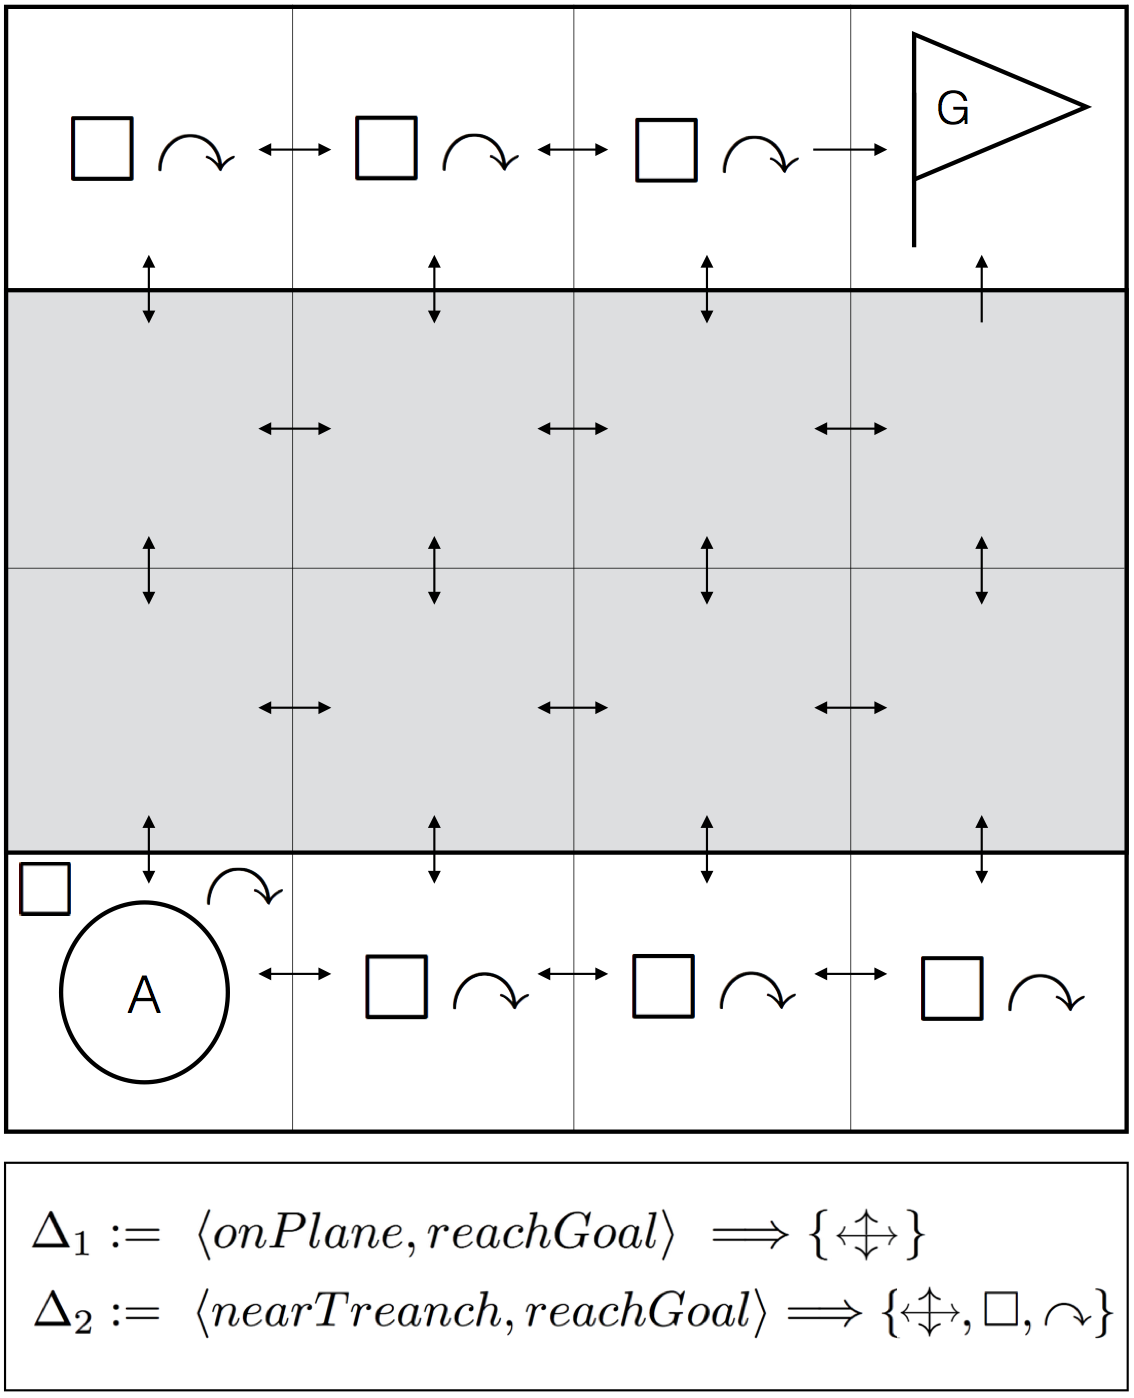
\includegraphics[scale=0.22]{figures/bridgeworld_aff.png}
%\caption{The affordance planner's state-action space on \texttt{BRIDGEWORLD}.}
%\label{fig:bridgeworld_aff}
%\end{figure}%

%Furthermore, given perfect subgoal knowledge for a
%particular planning task, the affordance formalism will find an
%optimal policy {\it extremely} quickly. We imagine extensions in which
%an agent gets stuck and must ask a human partner for help using
%natural language, and the resulting dialog could endow the agent
%with subgoal knowledge. This also allows the agent to prune way
%unnecessary actions in $\mathcal{A}$ in each specific planning task,
%making it possible to solve a engage with a large number of planning
%scenarios that may call for different actions. %
%

%% VI pseudocode + Affordances
%\begin{algorithm}
%  \caption{Affordance-VI($\mathcal{A}$, $\mathcal{R}$, $s_0$, $kb$, $goal$, $\epsilon$, $\gamma$) \\ {\it Complexity:} $\mathcal{O}(|\mathcal{A}|\cdot |\hat{\mathcal{S}}|^2)$}
%  \begin{algorithmic}[1]
%    \State $\hat{\mathcal{A}} \gets pruneActions(kb, s_0, \mathcal{A}, goal)$
%    \State $\hat{\mathcal{S}} \gets genStates(kb, \hat{\mathcal{A}})$
%    \While {$\delta < \epsilon \frac{(1-\gamma)}{\gamma}$}
%    \State $U \gets U';\delta \gets 0$
%    \For {each state $s \in \hat{\mathcal{S}}$}
%    \State $U'[s] \gets \mathcal{R}(s) + \gamma \max_{a \in \hat{\mathcal{A}}(s)} \sum_{s'} \text{Pr}(s'\mid s,a) U[s']$
%    \If {$|U'[s] - U[s]| > \delta$}
%    	\State $\delta \gets |U'[s] - U[s]|$ 
%    \EndIf
%    \EndFor
%    \EndWhile\\
%    \Return U;
%  \end{algorithmic}
%  \label{alg:aff_vi}
%\end{algorithm}%

%In the worst case, the Affordance-Value-Iteration Algorithm is 
%bounded by $\mathcal{O}(|\mathcal{A}|\cdot |\hat{\mathcal{S}}|^2)$, where
%$\hat{\mathcal{S}}$ is the subset of the states that were reachable using the
%resulting pruned action set determined by the agent's affordances. Thus,
%if the affordances were poorly designed, then the lower bound for the size of
%$\hat{\mathcal{S}}$, is precisely the full state space, $\mathcal{S}$. However,
%in general, when reasonable affordances are applied the agent is guaranteed to prune its
%action set for any number of states, and thus will explore less of the state space
%as a result.%

%The affordance formalism introduced above and expanded on in this
%paper resolves the weaknesses of these other frameworks by limiting
%the complexity of the seed knowledge required of the designer, while
%still providing enough knowledge to limit the search space but also
%maintain scalability.



\subsection{Subgoals}
\label{sec:subgoals}

\stnote{Subgoal planning drops right in as a third alternative
  framework we explore along with VI and rollout methods.  This
  section needs to be reorganized along these lines, where we define
  it, then say how it can benefit from affordances. }

Subgoal planning leverages the intuition that certain goals in
planning domains may only be brought about if certain preconditions
are first satisfied. For instance, in the bridge problem, one must
first place a block in the trench to create a bridge before crossing
the trench.  \citet{branavan12a} explore learning subgoals from the
Minecraft wiki and applying them in order to plan through a variety of
problems in Minecraft.

% Formalism
Formally, in subgoal planning, the agent is set of subgoals, where each subgoal is a pair of predicates:
\begin{align}
SG = \langle x_k, x_l \rangle
\end{align}

where $x_l$ is the effect of some action sequence performed on 
a state in which $x_k$ is true. Thus, subgoal planning requires 
that we perform high-level planning in subgoal space, and low-level 
planning to get from subgoal to subgoal. The low-level planner may vary, though
Metro-FF is a popular choice, as is Value Iteration.

\jmnote{I don't think it's necessary to include full pseudocode for the subgoal planning algorithm
since it is cited, but if it is included, the algorithm should probably be explained more in the text
(e.g., describe what subgoalKB means). Also, it seems like the subgoal space planner can
vary as well and doesn't need to be BFSs.}

% Subgoal planning pseudocode
\begin{algorithm}
  \caption{Plan with Knowledge Base of Subgoals \\ {\it Complexity:} $\mathcal{O}(|\mathcal{A}|\cdot |\mathcal{S}|^2)$}
  \begin{algorithmic}[1]
    \State subgoalSequence $\gets$ BFS(subgoalKB, goal)
    \State plan = []
    \State curState $\gets$ subgoalSequence.pop()
    \For {subgoal $\in$ subgoalSequence}
        \State plan += ValueIteration(curState, subgoal)
    \State curState $\gets$ plan.getLastState()
    \EndFor \\
    \Return plan;
  \end{algorithmic}
\end{algorithm}

In the case of \texttt{BRIDGEWORLD}, the agent might consider placing
a block somewhere along the trench to be a subgoal. Then, it runs
Value Iteration to get from its starting location to the subgoal.
Next, it runs Value Iteration from the first subgoal to the finish.
Subgoals enhance an agent's planning abilities when they propose {\it
  necessary} claims about the domain. If the subgoals are {\it
  contingent} (i.e. true in some state spaces of the domain but not in
others), then they do not limit the search space. For instance,
consider the task in \texttt{BRIDGEWORLD}, in which the agent must
place a block in the trench that separates the agent from the goal.
The subgoal $\langle blockInTrench, reachGoal\rangle$ might be a
perfectly useful subgoal in \texttt{BRIDGEWORLD}, but an adversary
could easily come up with thousands of worlds in which such a subgoal
would completely derail the agent's planner. Thus, many subgoals do
not scale beyond a particular instance of a state space. In order for
subgoals to be useful, they must be necessary claims about the domain,
otherwise, one can always come up with a counter world (by definition
of necessary).  Compare this scenario to the problem of baking bread
in minecraft: posessing wheat is always required to make bread, and it
is impossible to construct a world where this precondition is not
true.



{\bf Problem 2: Efficient Search} The last problem with subgoal
planning is that the use of subgoals actually requires that we
research a huge portion of the state space. Consider the
\texttt{BRIDGEWORLD} example in which the subgoal is to place a block
along the trench somewhere - once we plan from the state in which a
block has been placed at the trench, Value Iteration will search paths
exploring both sides of the trench rather than focusing on the
opposite side of the trench toward the goal.

\begin{figure}
\centering
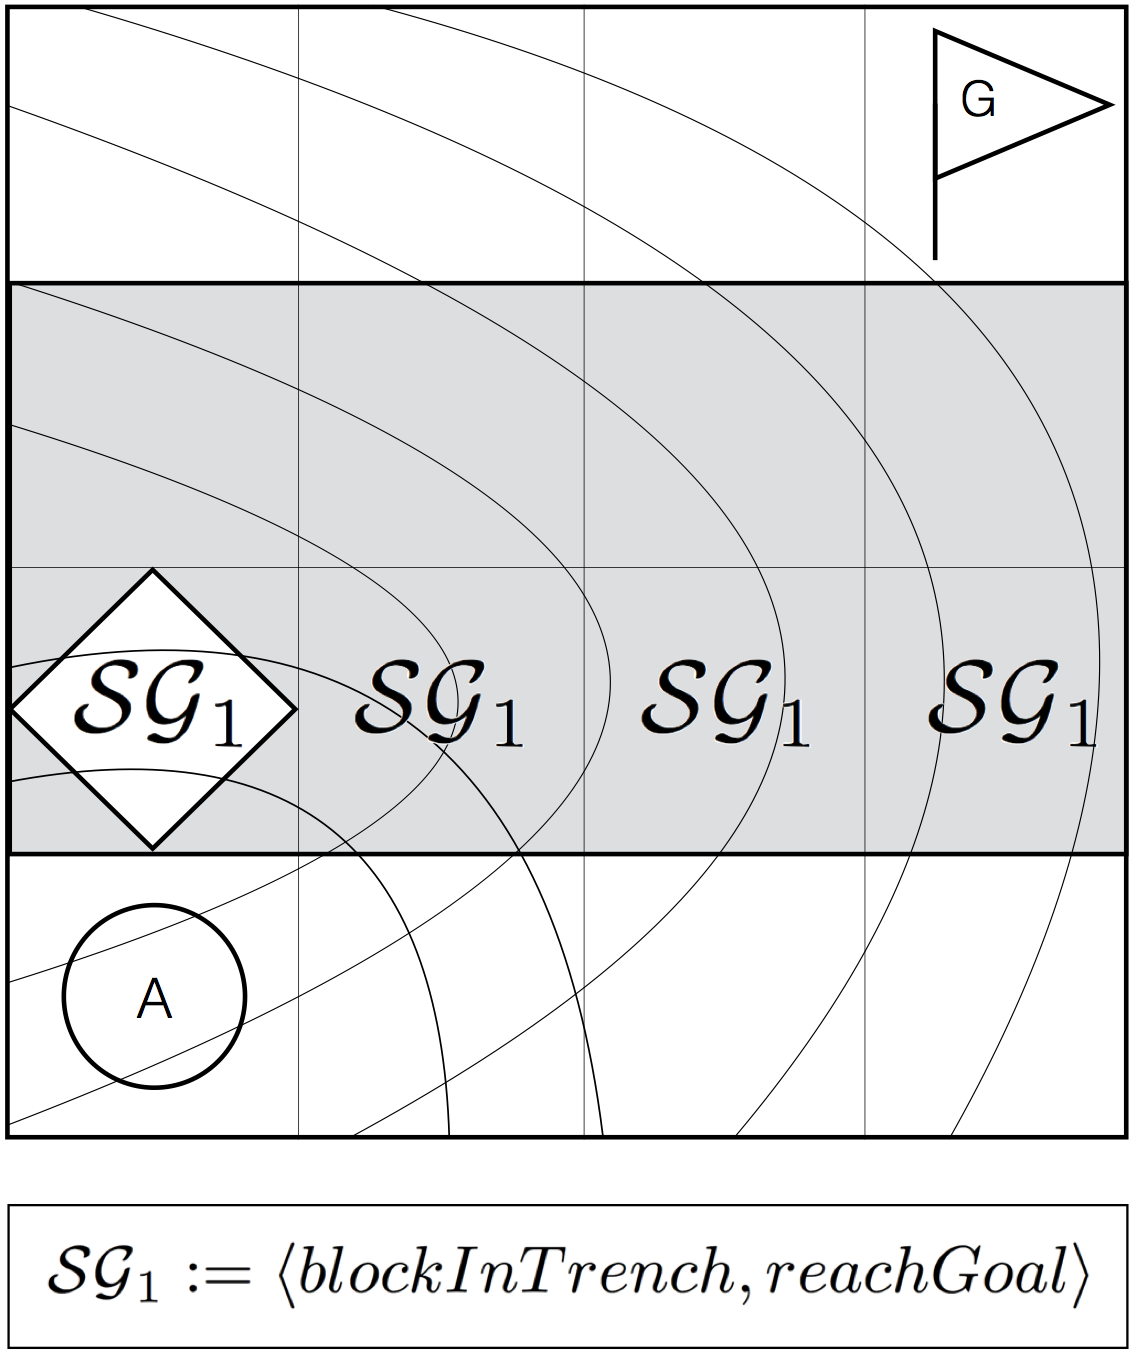
\includegraphics[scale=0.22]{figures/bridgeworld_sg.png}
\caption{The agent re-explores a large portion of the state space 
once it finds $\mathcal{SG}_1$. Also note that this subgoal 
highlights {\bf Problem 1}, in that it would be useless in many other Minecraft state spaces.}
\label{fig:bwsg}
\end{figure}


A final, but less significant problem, is that Subgoal planning still 
requires the use of Value Iteration or another low-level planner, which does not scale well - if 
there is ever a case in which planning between two subgoals is 
at all complex, then Subgoal planning is out of luck.






\section{EXPERIMENTS}

\jmnote{Reminder that this should be updated to be with respect to
  RTDP as a baseline and ideally should include a performance metric
  specifying the number of state backups that were used.}

\stnote{Experiments and results should be merged.  Also I think we
  need to think through how to structure the results. }

%\stnote{To write the experiments section, it's good to say what we are
%  interested in learning first.  What are we testing?  What is our
%  hypothesis?  Then explain the setup, then explain what the results
%  say about the hypothesis.  I would make experiments and results one
%  section, with subsections for each experiment + results}

We conducted a series of experiments in the Minecraft domain that
tested each planning system on a variety of tasks, ranging from basic
path planning, to baking bread, to opening doors and jumping over
trenches.  We also tested each planner on worlds of varying size to
demonstrate the scalability of each system. In Table \ref{results_1},
we provide results on testing the planners across each system. For
each data point, we ran the planning system 3 times and took the
average result (they rarely deviated beyond $\frac{1}{10}$ of a
second).

For the scenarios listed in Table \ref{results_1}, we limited the agent's 
action set across all planners so that it did not have access to block 
placement ($\square$) and block destruction ($\boxtimes$). The reason 
for excluding these two action types up is that, in Minecraft, the agent 
has an extraordinary ability to modify the state space via placing and 
destroying blocks. As a result, if an agent begins placing or destroying 
blocks in cases where it does not need to, the state-action space will 
explode exponentially and grow far too fast for (almost) any planner to 
finish in our lifetime. 


Equation \ref{eq:mc_explode} gives the order of the state space for a
$10\times10\times2$ Minecraft world,
%Consider that the agent is capable of destroying and placing blocks 
%in a 10x10x2 world; there are on the order of:%
%\begin{align}
%O\left(\sum_{n=1}^{10 \cdot 10 \cdot 2} \binom{10 \cdot 10 \cdot 2}{n}\right)
%\label{eq:mc_explode}
%\end{align}
which is far too large to explore. We will demonstrate that our 
affordance model {\it is} capable of handling these types of actions, 
and can plan using them as in a bridge building scenario or tunnel 
digging scenario (among others) while the other planners cannot. 
In fact, with these actions, none of the other planning systems 
can solve even the most basic path planning (even on just a flat 
surface with no obstacles). We explore this ability in the results 
seen in Table \ref{results_2}

As discussed above, one of the major advantages of using affordances 
to plan is that they enable an agent to have a massive action set, 
making affordances effectively transfer between domains. We 
conducted an additional set of experiments on the 15x15 world 
with no obstacles \texttt{15WORLD}. For this round of testing, we 
varied the number of actions available to the agent (starting from 
$|\mathcal{A}| = 4$ up to $|\mathcal{A}| = 25$) and ran the planner 
on \texttt{15WORLD} with the same goal (to reach the goal in the corner).


An additional advantage of planning with affordances is that the 
problems of block-placement and block-destruction illustrated by 
\ref{eq:mc_explode} are overcome. With affordances, we are able 
to solve a variety of novel planning problems in the Minecraft 
domain, such as building a bridge to cross a long trench, or digging 
a hole through a wall to reach the goal (see Table \ref{results_2}). 
This is indeed a compelling result, as no other planning system is 
currently able to avoid falling prey to the state-space explosion 
mentioned above. Additionally, the malleability of Minecraft that 
causes this explosion is a reasonable model of the way that an 
agent in the real world is capable of modifying its surroundings. 
Thus, we foresee the affordance planner as being extremely deft 
at handling real world planning scenarios.

\section{RESULTS}

\begin{table}
\begin{tabular}{ l || c | c | c }
  & Affordances & Subgoals & VI \\
  \hline
  \texttt{10WORLD} 		&	{\bf 0.6s} 		&	 1.8s 		& 1.1s  \\
  \texttt{13WORLD} 		&	{\bf 2.5s} 	 	& 	10.1s 		& 6.0s  \\
  \texttt{15WORLD} 		&	{\bf 6.7s} 	 	& 	21.6s 		& 11.8s  \\
  \texttt{17WORLD} 		& 	{\bf 16.6s} 	& 	45.4s 		& 28.2s  \\
  \texttt{20WORLD} 		& 	{\bf 57.6s} 	& 	144.3s 		& 140.5s  \\
  \texttt{JUMPWORLD}  	& 	{\bf 4.3s} 		& 	21.1s 		& 10.1s \\
  \texttt{BREADWORLD}  	& 	25.5s		& 	{\bf 22.8s} 	& 51.6s \\
  \texttt{DOORWORLD}  	& 	{\bf 16.3s} 	& 	25.0s 		& 25.3s \\
  \texttt{MAZEWORLD}  	& 	{\bf 17.9s} 	& 	114.8s		& 37.6s \\
  \texttt{HARDWORLD} 	& 	{\bf 34.5s}  	& 	215.9s 		& 149.7s
\end{tabular} 
\label{results_1}
\caption{Tests on a variety of tasks without block placement and destruction actions}
\end{table}

\vspace{4 mm}

\begin{table}
\begin{tabular}{ l || c | c | c }
  & Affordances & Subgoals & VI \\
  \hline
  $|\mathcal{A}| = 4$ 		& 	6.7s 	& 	11.8s 	& 6.7s  \\ % Just movement
  $|\mathcal{A}| = 8$ 		& 	6.8s 	& 	25.4s 	& 14.8s  \\ % + openDoor
  $|\mathcal{A}| = 12$ 	& 	6.8s 	& 	39.8s 	& 22.9s  \\ % + Oven
  $|\mathcal{A}| = 13$ 	& 	6.8s 	& 	41.28s      & 24.7s  \\ % + grain
  $|\mathcal{A}| = 17$ 	& 	6.7s	& 	55.5s	& 33.1s  \\ % + 0 blocks, placement
  $|\mathcal{A}| = 17$ 	& 	6.8s 	& 	DNF 		& DNF  \\ % + 1 blocks, placement
  $|\mathcal{A}| = 21$ 	& 	6.6s 	& 	DNF 		& DNF  \\ % + destruction
\end{tabular}
\label{results_2}
\caption{Plan on the simplest possible task (path planning in a flat plane with no obstacles - \texttt{15WORLD}) with incrementally larger action sets.}
\end{table}

\vspace{4 mm}

\begin{table}
\begin{tabular}{ l || c | c | c }
  & Affordances & Subgoals & VI \\
  \hline
  \texttt{BRIDGEWORLD} 		& 	? 	& 	DNF 		& DNF  \\
  \texttt{TUNNELWORLD} 		& 	? 	& 	DNF 		& DNF  \\
  \texttt{LADDERWORLD} 	& 	? 	& 	DNF 		& DNF  \\
  \texttt{TOWERWORLD} 		& 	? 	& 	DNF 		& DNF  \\
\end{tabular}
\label{results_2}
\caption{Bonus round: Minecraft specific tasks}
\end{table}


% Should explain DNF

As one can see from Table \ref{results_2}, in those cases where
$|\mathcal{A}| = 21$ and $|\mathcal{A}| = 25$, the only planning algorithm to
actually complete the tasks was the affordance planner. This is because each
of these cases scaled to include block destruction and block placement actions.
Thus, any case in which these actions are required to complete the task at hand,
only affordance planning will succeed. This is significant, as Table \ref{results_1}
indicates that the affordance planner plans more effectively than the other
systems, but it can also handle novel problems involving those actions that
alter the environment in sever ways.

We also include a Bonus round indicating
those tasks that only the affordance planner was able to solve. Finally, since
each affordance is attached to a particular goal, a single knowledge base will
scale across state-spaces and task types, causing affordance planning to be
extremely transferable. Additionally, we plan to add experiments in
Non-deterministic planning scenarios, as well as testing on the planning scenarios
from table \ref{results_1} where the knowledge bases remain constant across
state-spaces to test the generality of each algorithm.



% Insert bonus round of:
%	- Ladder!!!!
%	- Bridge
%	- Tunnel
%	- Builder tower under self



\section{Related Work}
In the past, numerous different forms of background knowledge have be used to 
accelerate planning algorithms. In section \ref{sec:subgoals}, subgoal
planning was discussed and in our experimental results, was compared against affordance-aware planning. 
In this section, we discuss the differences between affordance-aware planning and other
forms of background knowledge that have been used to accelerate planning.
Specifically, we discuss heuristics, temporally extended actions, and related action pruning work.


\subsection{Heuristics}
Heuristics in MDPs are used to convey information about the value of a given state or state-action pair with respect to the task being solved and typically take the form of either {\em value function initialization},
or {\em reward shaping}. For planning algorithms that estimate state-value functions, heuristics are often
provided by initializing the value function to values that are good approximations of the true value function. For example, initializing the value function to an admissible close approximation of the optimal value function has been shown to be effective for LAO* and RTDP, because it more greatly biases the states explored by the rollout policy to those important to the optimal policy~\cite{Hansen:1999qf}. Planning algorithms that estimate Q-values instead of the state value function may similarly initialize the Q-values to an approximation of the optimal Q-values. For instance, PROST~\cite{keller2012prost} creates a {\em determinized} version of a stochastic domain (that is, treating each action as if its most likely outcome always occurred), plans a solutions in the determinized domain, and then initializes Q-values to the value of each action in the determinized domain.

Reward shaping is an alternative approach to providing heuristics in which the planning algorithm uses a modified version of the reward function that returns larger rewards for state-action pairs that are expected to be useful. Reward shaping differs from value function initialization in that it may not preserve convergence to an optimal policy unless certain properties of the shaped reward are satisfied~\cite{potshap} that also have the effect of making reward shaping equivalent to value function initialization for a large class of planning/learning algorithms~\cite{Wiewiora:2003fk}.

A critical difference between heuristics and affordances is that heuristics are highly dependent on the task being solved; therefore, different tasks require different heuristics to be provided, whereas affordances are task independent and transferable between tasks. However, if a heuristic can be provided, the combination of heuristics and affordances may even more greatly accelerate planning algorithms than either approach alone.


\subsection{Temporally Extended Actions}

{\em Temporally extended actions} are actions that the agent can
select like any other action of the domain, except executing them
results in multiple primitive actions being executed in
succession. Two common forms of temporally extended actions are {\em
  macro-actions}%~\citep{hauskrecht98}
   \jmnote{looking at the citaiton you added for macros Stefanie, I think those are still ``options''
  rather than fixed primitive action sequences. Unfortunatley the term is overloaded a lot.}
  and {\em
  options}~\citep{sutton99}. Macro-actions are actions that always
execute the same sequence of primitive actions. Options are defined
with high-level policies that accomplish specific sub tasks. For
instance, when an agent is near a door, the agent can engage the
`door-opening-option-policy', which switches from the standard
high-level planner to running a policy that is hand crafted to open
doors. An option $o$ is defined as follows:

$o\ =\ \langle \pi_0, I_0, \beta_0\rangle$, where:

\begin{itemize}
\item[] $\pi_0 : (s,a) \rightarrow [0,1]$
\item[] $I_0 : s \rightarrow \{0,1\}$
\item[] $\beta_0 : s \rightarrow [0,1]$
\end{itemize}

Here, $\pi_0$ represents the {\it option policy}, $I_0$ represents
a precondition, under which the option policy may initiate, and 
$\beta_0$ represent the post condition, which determines which 
states terminate the execution of the option policy.

Although the classic options framework is not generalizable to different state spaces,
creating {\em portable} options is a topic of active research~\citep{konidaris07,konidaris2009efficient,Ravindran03analgebraic,croonenborghs2008learning,andre2002state,konidaris2012transfer}.

Although temporally extended actions are typically used
because they represent action sequences (or sub policies) that are often useful to solving
the current task, they can sometimes have the paradoxical effect
of increasing the planning time because they increase the number of actions that must be explored.
For example, deterministic planning algorithms that successfully make use of macro-actions often avoid the potential increase
in planning time by developing algorithms that restrict the set of macro-actions to a small set that is expected to improve planning time~\cite{Botea:2005kx,Newton:2005vn} or by limiting the use of macro-actions to certain conditions
in the planning algorithms like when the planner reaches heuristic plateaus (areas of the state space in which all child states have the same heuristic value)~\cite{Coles:2007ys}. Similarly, it has been shown that the inclusion
of even a small subset of unhelpful options can negatively impact planning/learning time~\cite{Jong:2008zr}.

Given the potential for unhelpful temporally extended actions to negatively impact planning time, we believe combing affordances with temporally extended actions
may be especially valuable, because it will restrict the set of temporally extended actions to those
which may actually be useful to a task. In the future, we plan to more directly explore the benefit from combining
these approaches.


%Recently, Konidaris and Barto's ~\citep{konidaris07} 
%expand on the classic options framework and allow for a more portable 
%implementation of options. Still, though, planning with options requires either 
%that we plan in a mixed space of actions {\it and} options (which blows up the 
%size of the search space), or requires that we plan entirely in the space of options. 
%Additionally, providing an agent with an option policy is a difficult task for a human 
%designer (especially if we want an optimal policy, which we do).

\subsection{Action Pruning}
\jmnote{We should also probably do a search for other MDP action pruning approaches, just to
make sure we're not missing anything especially important.}

Perhaps the most similar work to ours is Sherstov and Stone's action transfer work~\cite{sherstov2005improving}.
In their work, they considered MDPs with a very large action set and for which the action
set of the optimal policy of a source task could be transferred to a new, but similar, target
task to reduce the learning time required to find the optimal policy in the target task. Since the actions
of the optimal policy of a source task may not include all the actions of the optimal policy
in the target task, source task action bias was reduced by randomly perturbing the value function
of the source task to produce new synthetic tasks. The action set transferred to the target task
was then taken as the union of the actions in the optimal policies for the source task and all the
synthetic tasks generated from it.

A critical difference between our affordance-based action set pruning and this action transfer
work is that affordances represent knowledge defined independently of any specific task. Therefore,
affordances can be defined once and reused in a variety of very different tasks, whereas in the action transfer work, action set pruning
must begin anew when the current task is very dissimilar from previously experienced tasks.

\jmnote{Do we want to make any comments about how this work might be useful in future work that learns
affordances rather than is given them?}



\section{CONCLUSION}
\jmnote{Will probably need to update this to reflect changes in paper.}

We proposed a novel approach to representing knowledge in terms of
{\em affordances}~\citep{gibson77} that allows an agent to efficiently
prune its action space based on domain knowledge. This pruning was
shown to significantly reduce the number of state/action pairs the
agent needs to evaluate in order to act optimally, and resulted in
faster planning than subgoal planning, options, and vanilla value
iteration. We demonstrated the efficacy as well as the transferability
of the affordance model in a series of planning tasks in the Minecraft
domain.

In the future, we hope to learn affordances from experience as opposed
to providing them directly to the agent. Additionally, we hope to
introduce uncertainty into the action set that is pruned, in order to
improve the effectiveness of the pruning. Lastly, we hope to
incorporate aid from a human partner through natural language
dialogue, in which the agent may ask for help when it is stuck and
receive subgoal {\it hints} from a human companion.

\bibliographystyle{plainnat}
\bibliography{main}  


\end{document}
